\section{Results and Discussion}\label{sec:results}
% Required: how the experiments were run, what varied between the generated songs, the
% fitness graph, links to the audio, and a qualitative discussion.
% About 1 column plus the figures.

\subsection{Experimental Setup}
% Setup: mutation rate 0.01, 0.05 and 0.2, seeds 1, 2 and 3, all other parameters at the
% default (Table~\ref{tab:params}). Reproduce with ./experiments.sh and python compare.py.
% Audio: runs/experiments/<run>/audio/gen_1249.wav in the repository.
TODO

\subsection{Fitness Evolution}
% Points to discuss (check them against Figures~\ref{fig:fitness} and \ref{fig:comparison}
% and Table~\ref{tab:results}):
% - 0.01 ends at 0.999 on all 3 seeds.
% - 0.05 ends between 0.91 and 0.99 (average 0.95).
% - 0.2 stalls around 0.64 to 0.70.
% - The mean fitness stays far below the best (about 0.58 at 0.05).
TODO

\subsection{Listening Analysis}
% Qualitative discussion (required): what sounds different between the songs of each
% mutation rate and seed. Does a fitness near 1.0 sound good, or repetitive?
TODO

\subsection{Limitations and Future Work}
% Limitations to consider: fixed progression and key, only eighth notes, equal weights chosen
% by hand, fitness measures rule compliance and not musical quality, no listening test.
% Extensions: other progressions, rhythmic variety, tuning the weights, a listening study,
% interactive fitness as in GenJam \cite{biles1994}.
TODO

\begin{figure}
  \centering
  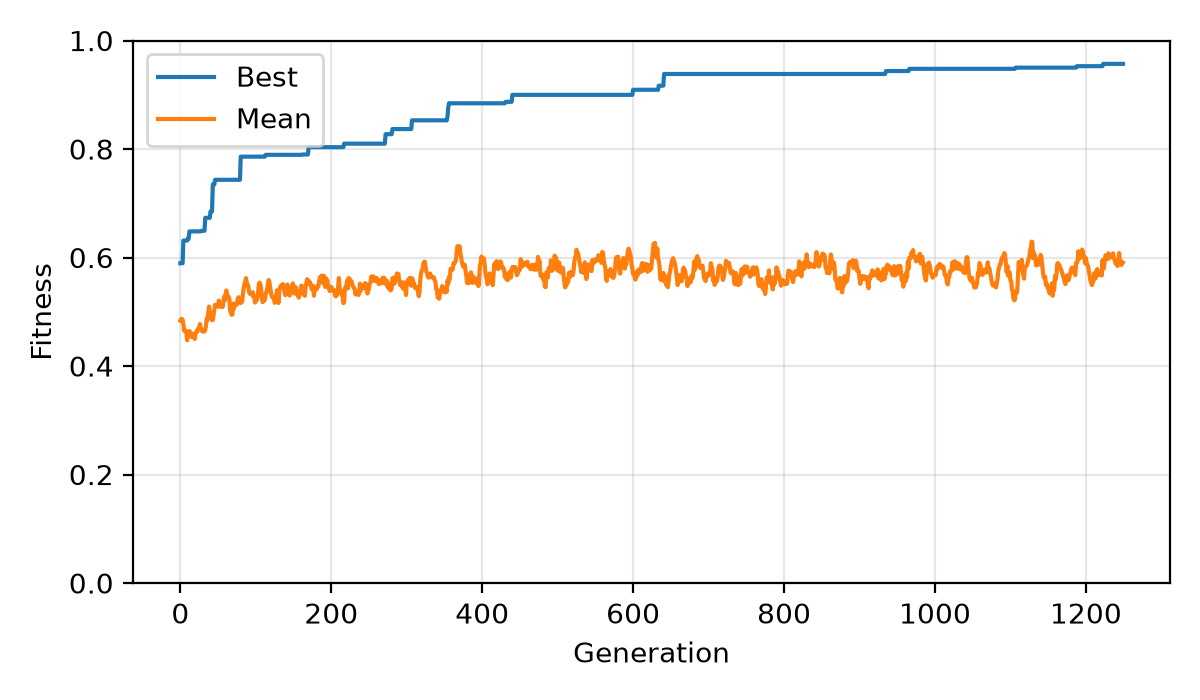
\includegraphics[width=\linewidth]{figures/fitness.png}
  \caption{Best and mean fitness per generation for the default configuration
    (mutation rate 0.05, seed 1).}
  \label{fig:fitness}
\end{figure}

\begin{figure}
  \centering
  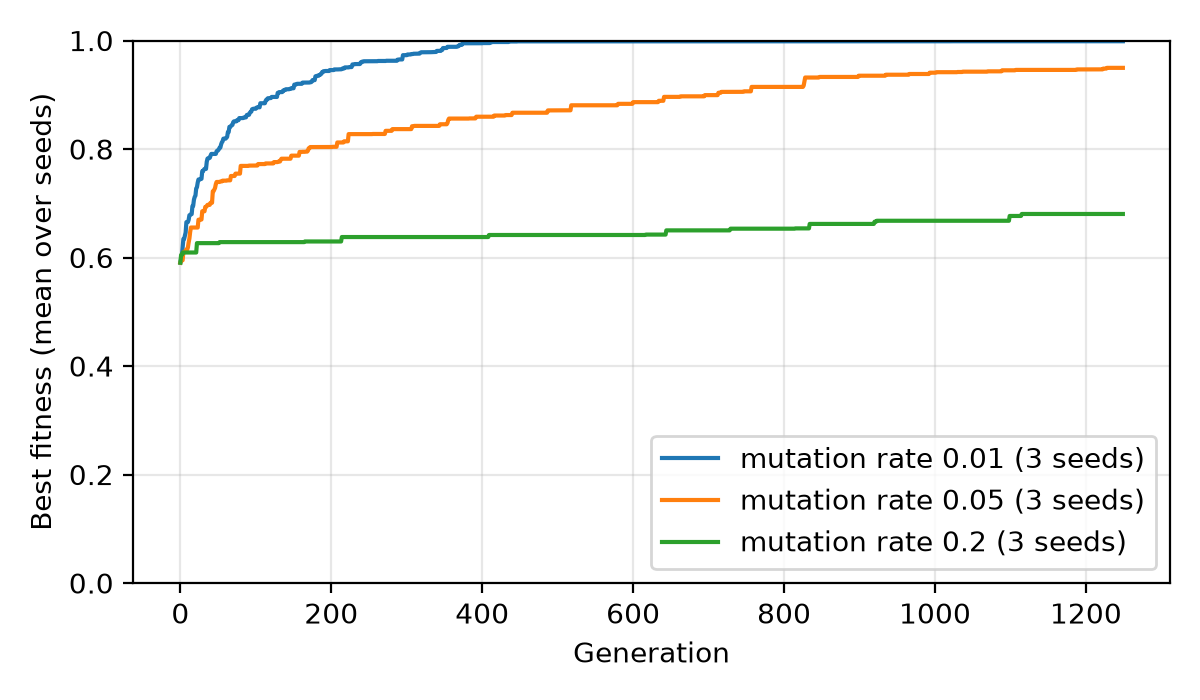
\includegraphics[width=\linewidth]{figures/comparison.png}
  \caption{Best fitness per generation for each mutation rate, averaged over 3 seeds.}
  \label{fig:comparison}
\end{figure}

\begin{table}
  \centering
  \begin{tabular}{lcccc}
    \toprule
    Rate & Seed 1 & Seed 2 & Seed 3 & Mean \\
    \midrule
    0.01 & 0.999 & 0.999 & 0.999 & 0.82 \\
    0.05 & 0.957 & 0.986 & 0.906 & 0.58 \\
    0.2  & 0.704 & 0.644 & 0.693 & 0.39 \\
    \bottomrule
  \end{tabular}
  \caption{Best fitness at the last generation (1249) per mutation rate and seed, and
    population mean fitness
    averaged over the 3 seeds.}
  \label{tab:results}
\end{table}
